\section{Tactical combat - Battlescape}

So this is where all the fun happens ;) It is here that your former choices have to proof their worth as well as you will have to prove your commanding skills.
The goal of every tactical combat is quite simple: kill all those evil aliens with as few civilian (and of cause squad) looses as possible. In order to achieve this you will have to find a good balance between caution and fast proceedings. You don't want to watch all innocents die like flies just because your soldiers are afraid of the enemy.
In the course of the game you will see a wide range of settings and environments, but no matter how bad things may look like, there a some quite powerful tools at you hand to get rid of them. If you have some experience with (turn-based) tactical combat games you should find some redundant elements - and of cause you will if you ever played any other UFO before. Nevertheless you should take a short overview over the interface so you make sure you don't miss any important feature. To change the view within battlescape you may use either cursor buttons or \keybinding{WASD}. Please be aware that its also possible to change the pitch of the camera. (\keybinding{R} and \keybinding{F} by default)
There are two alternative interfaces available right now, offering identical functions of cause. In the following we will discuss bot of them. You may switch between them as often as you want until you feel familiar with one of them (options $\hookrightarrow$ game).
While the first one is heavily inspired by the classic HUD the second one (althud) tries to utilise modern techniques to achieve cleaner optics.

\subsection{Buttons - HUD}
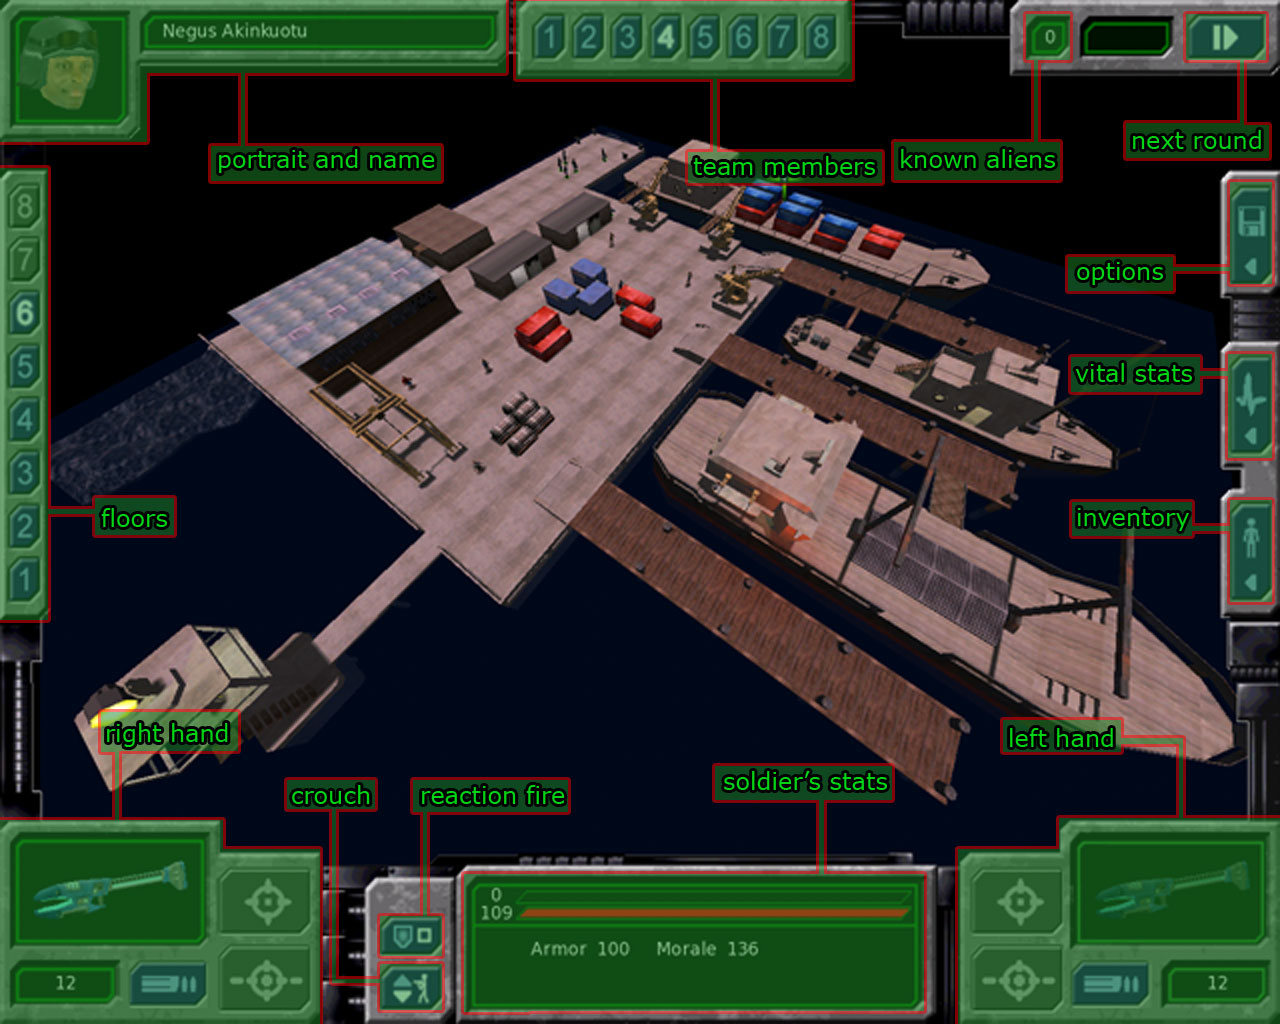
\includegraphics[width=\textwidth]{images/HUD_final.jpg}
\subsubsection{Floors}
Here you can change the ``ground-level'' or floor shown in the tactical view. Besides its obvious use in order to move you soldiers between different floor-levels it's also helpful to get an general overview. So it's always a smart move to switch between all levels at the beginning of each mission so you won't miss the ``hidden'' cellar or rooftop.
\subsubsection{Portrait and name}
This is more for aesthetic reasons, so no big actions are bound to this. (But of cause - as usual- suggestions are welcome)
\subsubsection{Team-members}
There is where you can switch between you soldiers (alternatively use keybindings: 1 to 8 or just left-click on their model). In case one (or more *G*) of your devoted fighters lost their live fighting the evil his button will become grey.
\subsubsection{Known aliens}
This states the number of aliens all your squad member have discovered this round. By clicking on it you may switch through all of them.
\subsubsection{Next round}
Hmm... so what do you suspect this one does? Exactly!
\subsubsection{Options}
Opens the ``Options''-menu where you may vary several video/sound-settings as well as abort or retry current missions. Be aware that it's not possible nor intended to save a ongoing mission. If you abort the current mission, all your soldiers will be lost.
\subsubsection{Vital stats}
This is where you find more detailed information about health, moral and psi-power of your soldier.
\subsubsection{Inventory}
Opens the inventory of the selected soldier. This is where you can change weapons, pick up/drop items or just take a look at your great heroes.
\subsubsection{Soldiers stats}
This is a summery of all general information you need to use your soldier most efficiently. Its content interacts with your mouse action, but should be quite self-explaining. Not only you will find health and remaining TUs (we will deal with TUs in the following section) here but also it will give you the amount your currently selected shooting-mode will consume as well as some other info's like current armor and moral.
\subsubsection{Reaction fire}
This button enables ``reaction fire'', a central concept of every tactical combat. We will deal with it in the following chapter. For now you should just remember that it is here where you turn it on and off.
\subsubsection{Crouch}
As one might guess, this button will make your soldier kneel down (and by doing so reducing the danger of being hit by enemy fire) or if he already does make him stand up. Please notice that a soldier that kneels down can still move forward as if he would stand upright, but it takes him 1 additional time unit per square to do so.
\subsubsection{Right/left-hand}
Those two fields are completely identical besides the fact the left hand one is active only if you actually wear two one-handed items/weapons. If you have a two-handed item/weapon equipped the left-hand field will be inactive. Because each of the two fields consist of several important buttons itself we will discuss them a bit more detailed. Please take a look at the following image.\\
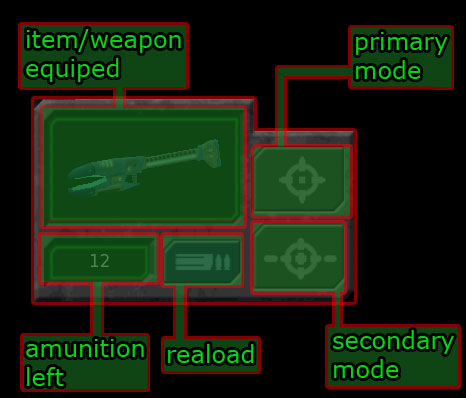
\includegraphics[width=6cm]{images/HUD_detail_final.jpg}
%as float ?!
%transparent background ?! ->going to be re-worked soon
\subsubsection{Item/weapon}
Gives a picture of the currently equipped item/weapon. This turns red in case you can't use the weapon, for example because you don't know the tech or don't have any ammunition left.
\subsubsection{Primary-mode}
Activates primary-mode for this item. In case of weapons this is usually (but not always!) a fast but less accurate / powerful shoot. For details see weapon description.
\subparagraph{Secondary-mode}
Activates secondary-mode for this item. In case of weapons this is usually (but again, not always!) a more TU-consuming but also more accurate / powerful shoot. Please notice that in case the item supports only one mode (like stun rod) both modes are identical.
\subsubsection{Reload}
Reloads currently equipped weapon, if ammunition is left in the inventory.
\subparagraph{Ammunition left}
Shows the ammunition left in your weapon. Please notice that some shooting-modes (also some of the one-shoot ones) require more than one ``bullet'' here.

\subsection{Buttons - altHUD}

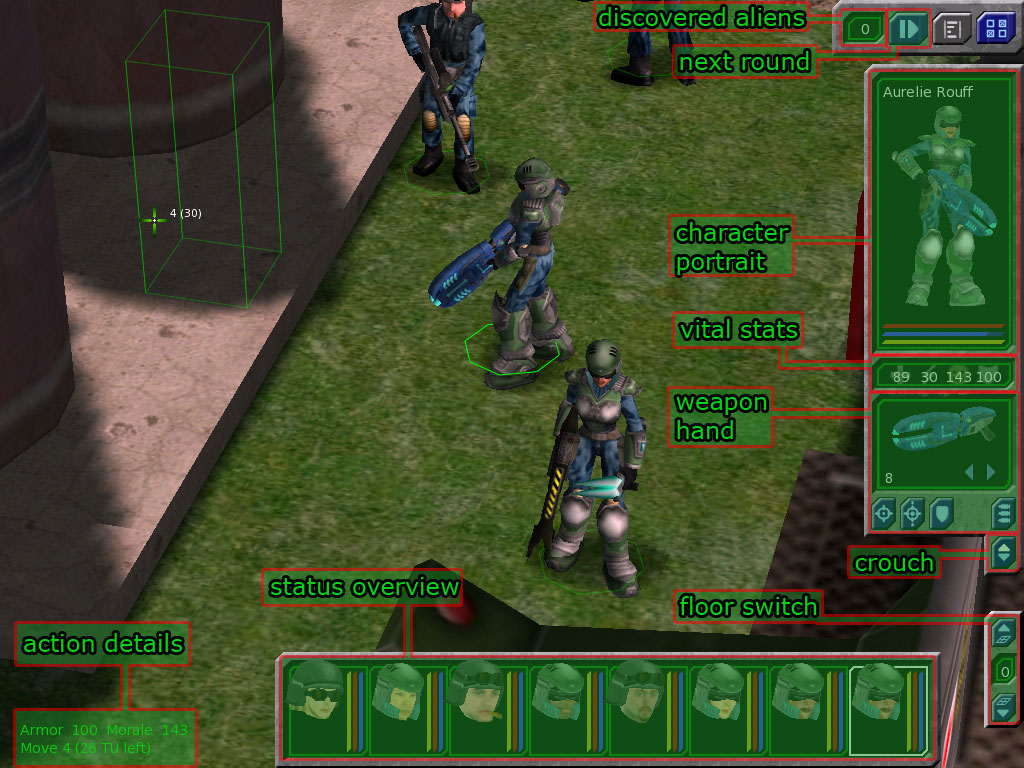
\includegraphics[width=\textwidth]{images/altHUD_final.jpg}\\

\subsubsection{Discovered aliens}
This states the number of aliens all your squad member have discovered this round. By clicking on it you may switch through all of them.
\subsubsection{Next round}
Hmm\ldots so what do you suspect this one does? Exactly!
\subsubsection{Options}
Opens the ``Options''-menu where you may vary several video/sound-settings as well as aboard or retry current missions. Be aware that it's not possible nor intended to save a ongoing mission.
\subsubsection{Character portrait}
Besides giving you the chance to admire your well dressed and equipped soldiers clicking on a soldiers portrait opens up his or her inventory.
\subsubsection{Vital stats}
This is where you find more detailed information about (from left to right) health, remaining TUs, moral and armor of your soldier.
\subsubsection{Action details}
Here some more details on your current action are displayed. If you are about to move your soldier this means you will be shown the required TU costs as well as how many will be left (if any) at the end of this action. In case you have selected one of the two firemodes you will be informed about the TU costs and the approximate probability to hit the target. Hint: Even with an 100\% chance it is still possible (but very unlikely) that your soldier failed to hit the target for unforeseeable  reasons.
\subsubsection{Crouch}
As one might guess, this button will make your soldier kneel down (and by doing so reducing the danger of being hit by enemy fire) or if he already does make him stand up. Please notice that a soldier that kneels down can still move forward as if he would stand upright, but it takes him 1 additional time unit per square to do so.
\subsubsection{Floor switch}
Here you can change the ``ground-level'' or floor shown in the tactical view. Besides its obvious use in order to move you soldiers between different floor-levels it's also helpful to get an general overview. So it's always a smart move to switch between all levels at the beginning of each mission so you won't miss the ``hidden'' cellar or rooftop.
\subsubsection{Status overview}
There is where you can switch between you soldiers (alternatively use keybindings: \keybinding{1} to \keybinding{8} or just left-click on their model). In case one (or more *G*) of your devoted fighters lost their life fighting the evil, his button disappears. Three different ??? give you an fast overview over your teams vital statistics. Red representing health points, yellow moral and blue the amount of remaining time units.
\subsubsection{Weapon hand}
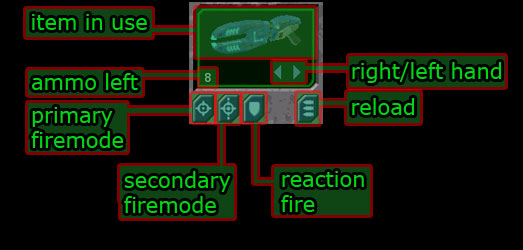
\includegraphics[width=6cm]{images/altHUD_detail_final.jpg}

\subsubsection{Weapon in use}
Gives a picture of the currently equipped item/weapon. This turns red in case you can't use the weapon, for example because you don't know the tech or don't have any ammunition left.
\subsubsection{Ammo left}
Shows the ammunition left in your weapon. Please notice that some shooting-modes (also some of the single shot ones) require more than one ``bullet'' here.
\subsubsection{Primary firemode}
Activates primary-mode for this item. In case of weapons this is usually (but not always!) a fast but less accurate / powerful shoot. For Details see weapon description.
\subsubsection{Secondary firemode}
Activates secondary-mode for this item. In case of weapons this is usually (but again, not always!) a more TU-consuming but also more accurate / powerful shot. Please notice that in case the item supports only one mode (like stun rod) both modes are identical.
\subsubsection{Reaction fire}
This button enables ``reaction fire'', a central concept of every tactical combat. We will deal with it in the following chapter. For now you should just remember that it is here where you turn it on and off.
\subsubsection{Reload}
Reloads currently equipped weapon, if ammunition is left in the inventory (consumes TUs).
\subsubsection{Right/left hand}
Switches between the left and right hands item (in case the soldier carries two one handed items).

\section{Game-mechanics (Battlescape)}

\subsection{Time-units (TUs)}
As mentioned before every soldier has a certain amount of time units (TUs) which are mainly determined by his ``speed'' attribute. Every action done by him costs a varying amount of TUs this holds for firing or reloading a weapon as well as walking or re-equipping him in the inventory. The amount of TUs needed for using the primary/secondary mode is given in the status window after selecting one of the two.

\subsection{Movement}
Like firing a weapon, movement also consumes time units. You can make your soldier walk to a spot using your mouse on the tactical view. You will notice that your cursor turns to a green square indicating that this place is reachable with your current amount of TUs or turn blue if it is not (this might be the case due to a lack of TUs or for geographical reasons). If the square is green it will also prompt two numbers of which the first one states the TU-cost of this movement while the second one represents your actual amount of TUs. In case your soldier notices a new enemy or civilian in his line of sight while walking the movement will be interrupted, giving you the chance to adjust your orders according to this new situation.

\subsection{Line of sight}
For obvious reasons you soldiers, in general, can only shoot at what they see. After finishing an ordered movement your soldier will look in the direction of his last step, which is not very helpful in a lot of situations. To solve this you might make use of the possibility to change your soldiers viewing direction. This can be done in different ways, e. g. \keybinding{Right-mouse-button} / \keybinding{CTRL}. For details please refer to your keybindings in the game options menu.

\subsection{Shooting-modes}
As we have said before most items, weapons in particular, do have two different action/firing-modes. While the second firing-mode of a sniper rifle is an aimed shot, some assault rifles can start a long fireburst or fire one concentrated and by that devastating single beam. Whatever weapon raises you interest, Ufopedia is your friend. If you look up a certain weapon like that you might be confused, the only information that can be found here is its name and if its a two-handed one or not. What seems rather wired on first sight has a simple reason. As some weapons can be equipped with a wide range of different kinds of ammunition their use and stats also heavily depend on the ammunition loaded. So once you look up the ammunition you want to use you will find all the data and statistics you are looking for - given you have done the required research. Doing so you will find that different firing-modes not only differ by TU needed and damage done but also by weapon skills needed.

\subsection{Close combat}
An alien is popping up just around the corner and not enough TUs left to fire this Plasma-Blaster in secondary mode while primary-mode offers only indirect fire? Your soldiers being keen on some extra thrill? You want to capture an living alien for ``interrogation'' but all your research department has to offer is a stun rod of which they say it might work --- somehow\ldots? No matter what the reasons may be, there will be a time you will get into close-combat, or it will get to you. While the reason to be that close to an hostile alien might be quite scary, lucky enough the way to use the interface in such a situation is not at all. Overall it works exactly like caring a gun besides the fact that your power skill is taken into consideration when calculating the combat results. Also most close combat weapons (that includes pistols as well) do have a far more devastating impact on their target compared for their needed TUs making them a reasonable choice in small and narrow environments like buildings and the likes. Hint: Most pistols also fall under the close combat category which makes them a useful alternative.

\subsection{Friendly fire}
You better make sure there is no one of your soldiers in any possible line of fire when using RF or normal firemodes - friendly fire is rather strict right now.

\subsection{Reaction fire}
One of the main aspects every experienced commander needs to be able to use for his advantage is what is called ``reaction fire'' (RF). When discussing the basics of battlescape we already mentioned its button but spared to explain the corresponding concept. To make things even more complicated there are two kinds of reaction fire (referred to RF-1 or RF-2 in the following). The RF-mode that is activated is indicated by one or two $\surd$ s (HUD) or an ``i'' or ``*'' (altHUD). When enabled (costing a certain amount of TUs) your soldier will be able to react on new situations and sightings after you already ended your turn. For doing so in case of RF-1 he has one shot on any enemy that he has at least a 30\% chance to hit with no more than 5\% risk of friendly fire. Those conditions also hold for RF-2 but with this option the soldier in question fires as often as possible while he has all the TUs of the upcoming round (without costs for RF) at his disposal to fire his weapon in order to deal with this more or less surprising situation. Especially after having suffered heavy penetration by enemy fire with reaction-fire activated, your soldiers will refuse your order to ``turn it off'' as they are too scared to let their guard down or will take greater risks (lesser chance to hit or bigger tolerance to friendly fire) in their approach to kill the enemy. For details about this and other effects of a bad moral please refer to the according section of the manual.

\subsection{Damagetypes}
Obviously different weapons cause different kinds of damage. To reflect this fact each weapon is assigned a certain damage-class. This gets important when it comes to armor types as different armor types suit different damage types. Details can be found in the according armor and ammunition Ufopedia entries. This way it might be possible that some armor that is almost impenetrable for plasma damage fails to offer any protection against weapons that inflict fire damage.

\subsection{Stun}
In order to find out more about your alien enemy and his goal, motivation and structures you might find it useful to catch one or more them for direct interrogation. Once your research lab developed the tools needed to do so you might use them as any other weapon of this kind (e.g. grenades, close-combat, etc.). After successfully finishing a mission those stunned alien will be brought to your base. Please be aware that you will need special structures to make sure your ``guest'' will stay long enough to give you any answer at all. If you lack those facilities your stunned aliens will die instantly once you've reached your base. In case everything is prepared to make your stunned aliens feel at home they will open up new options in the research department.

\subsection{Morale}
Your squads, but also your enemies, morale plays an important role in tactical combats. Especially in critical situations that tend to bring the decision on win or lose.\\
There are a couple of influences to any characters moral and once one reaches a critical point the result can be anything from throwing away your weapon and running away to panic attacks including shooting at allied forces.\\
A characters moral is going to drop slightly when is witnesses a civilian being killed. If the same happens to a squadmember his moral drop far more remarkable and if an alien dies nearby on the other hand moral is going to increase. All that relative to the soldiers moral values.
